\documentclass[a4paper,twoside]{article}   
\usepackage{amsmath,amssymb,amsfonts}
\usepackage{graphics}
\usepackage{epsfig}
% 
%  
% Please submit at http://www.easychair.org/conferences/?conf=ttc2011. Your submission should include (i) a case description (in PDF format) answering the above questions, (ii) a ZIP archive that contains all test artifacts, and (iii) an evaluation scheme (a spreadsheet file or a pointer to an online "classification scheme").

\begin{document}

\title{Submission for Transformation Tool Contest 2011: Sample URDAD model}

\author{ Fritz Solms, Craig Edwards and Stefan Gruner\\
  {\small Dept. of Comp. Science, University of Pretoria, email: fritz@solms.co.za, sgruner@cs.up.ac.za}}

\maketitle

%\begin{abstract}
Use-Case Responsibility-Driven Analysis and Design (URDAD) is a service-oriented software analysis and design methodology. It is used by requirements engineers to develop technology-neutral, semi-formal platform-indepen\-dent models (PIM) within the OMG's MDA. In the past, URDAD models were denoted in UML. However, that was tedious and error-prone. The resulting models were often of rather poor quality. In this paper we introduce and discuss a new Domain-Specific Language (DSL) for URDAD. Its meta model is consistent and satisfiable. We show that URDAD DSL specifications are simpler and allow for more complete service contract specifications than their corresponding UML expressions. They also enable traceability and test case generation.
\end{abstract}


\tableofcontents

\section{Contextualization}

URDAD, the {\em Use-Case, Responsibility-Driven Analysis and Design} \cite{solms_urdad_2010, solms_generating_2009, solms_technology_2007} method, is a method used by requirements specialists (typically business analysts) to perform technology neutral, services oriented analysis and business process design. The resultant analysis and business process design models are meant to be augmented by technical experts to formalize conditions and constraints.

The output of the URDAD method is an URDAD model containing the requirements and technology neutral process design. Historically the URDAD model has been encoded in UML. Such an encoding suffers from impresice semantics, excessive model complexity and high model defect rates caused by the size and complexity of UML and the high level of discipline required to encode an URDAD model in UML.

To address these issues and metamodel introducing only the URDAD model features has been developed. This metamodel forms the basis for a {\em Domain-Specific Language} (DSL) for URDAD.  The model is meant to be populated through the use of concrete text and diagrammatic syntaxes defined for the URDAD DSL. Currently a concrete EMFText-based syntax is available.

An URDAD model recursively assembles higher level services from lower level services. The leaf services are services sourced from the environment. These include services provided by the implementation language/technologies, persistence services and services sourced from external systems. For each service the the URDAD model contains
\begin{itemize}
 \item the \textit{service contract} with data structure specification for the request (input) and result (output) object as well as pre- and post-conditions used for functional testing and quality requirements used for testing non-functional requirements,
 \item the \textit{service} specification specifying the functional requirements (i.e.\ lower level services from which this higher level service is assembled), and the actual orchestration of the process for the service across these lower level services. The outcome of the service is either the result object (return value) or the notification that the service is not provided due to a particular pre-condition not having been met by raising the exception for that pre-condition.
\end{itemize}

\subsection{The URDAD meta-model}

The URDAD metamodel specifies the model structure for the input model of the transformation. It is encoded in Ecore and is encluded in the artifacts provided to the mapping teams. Figure \ref{fig:metamodel} shows a diagrammatic representation of the metamodel. 

\begin{figure}
  \centering
  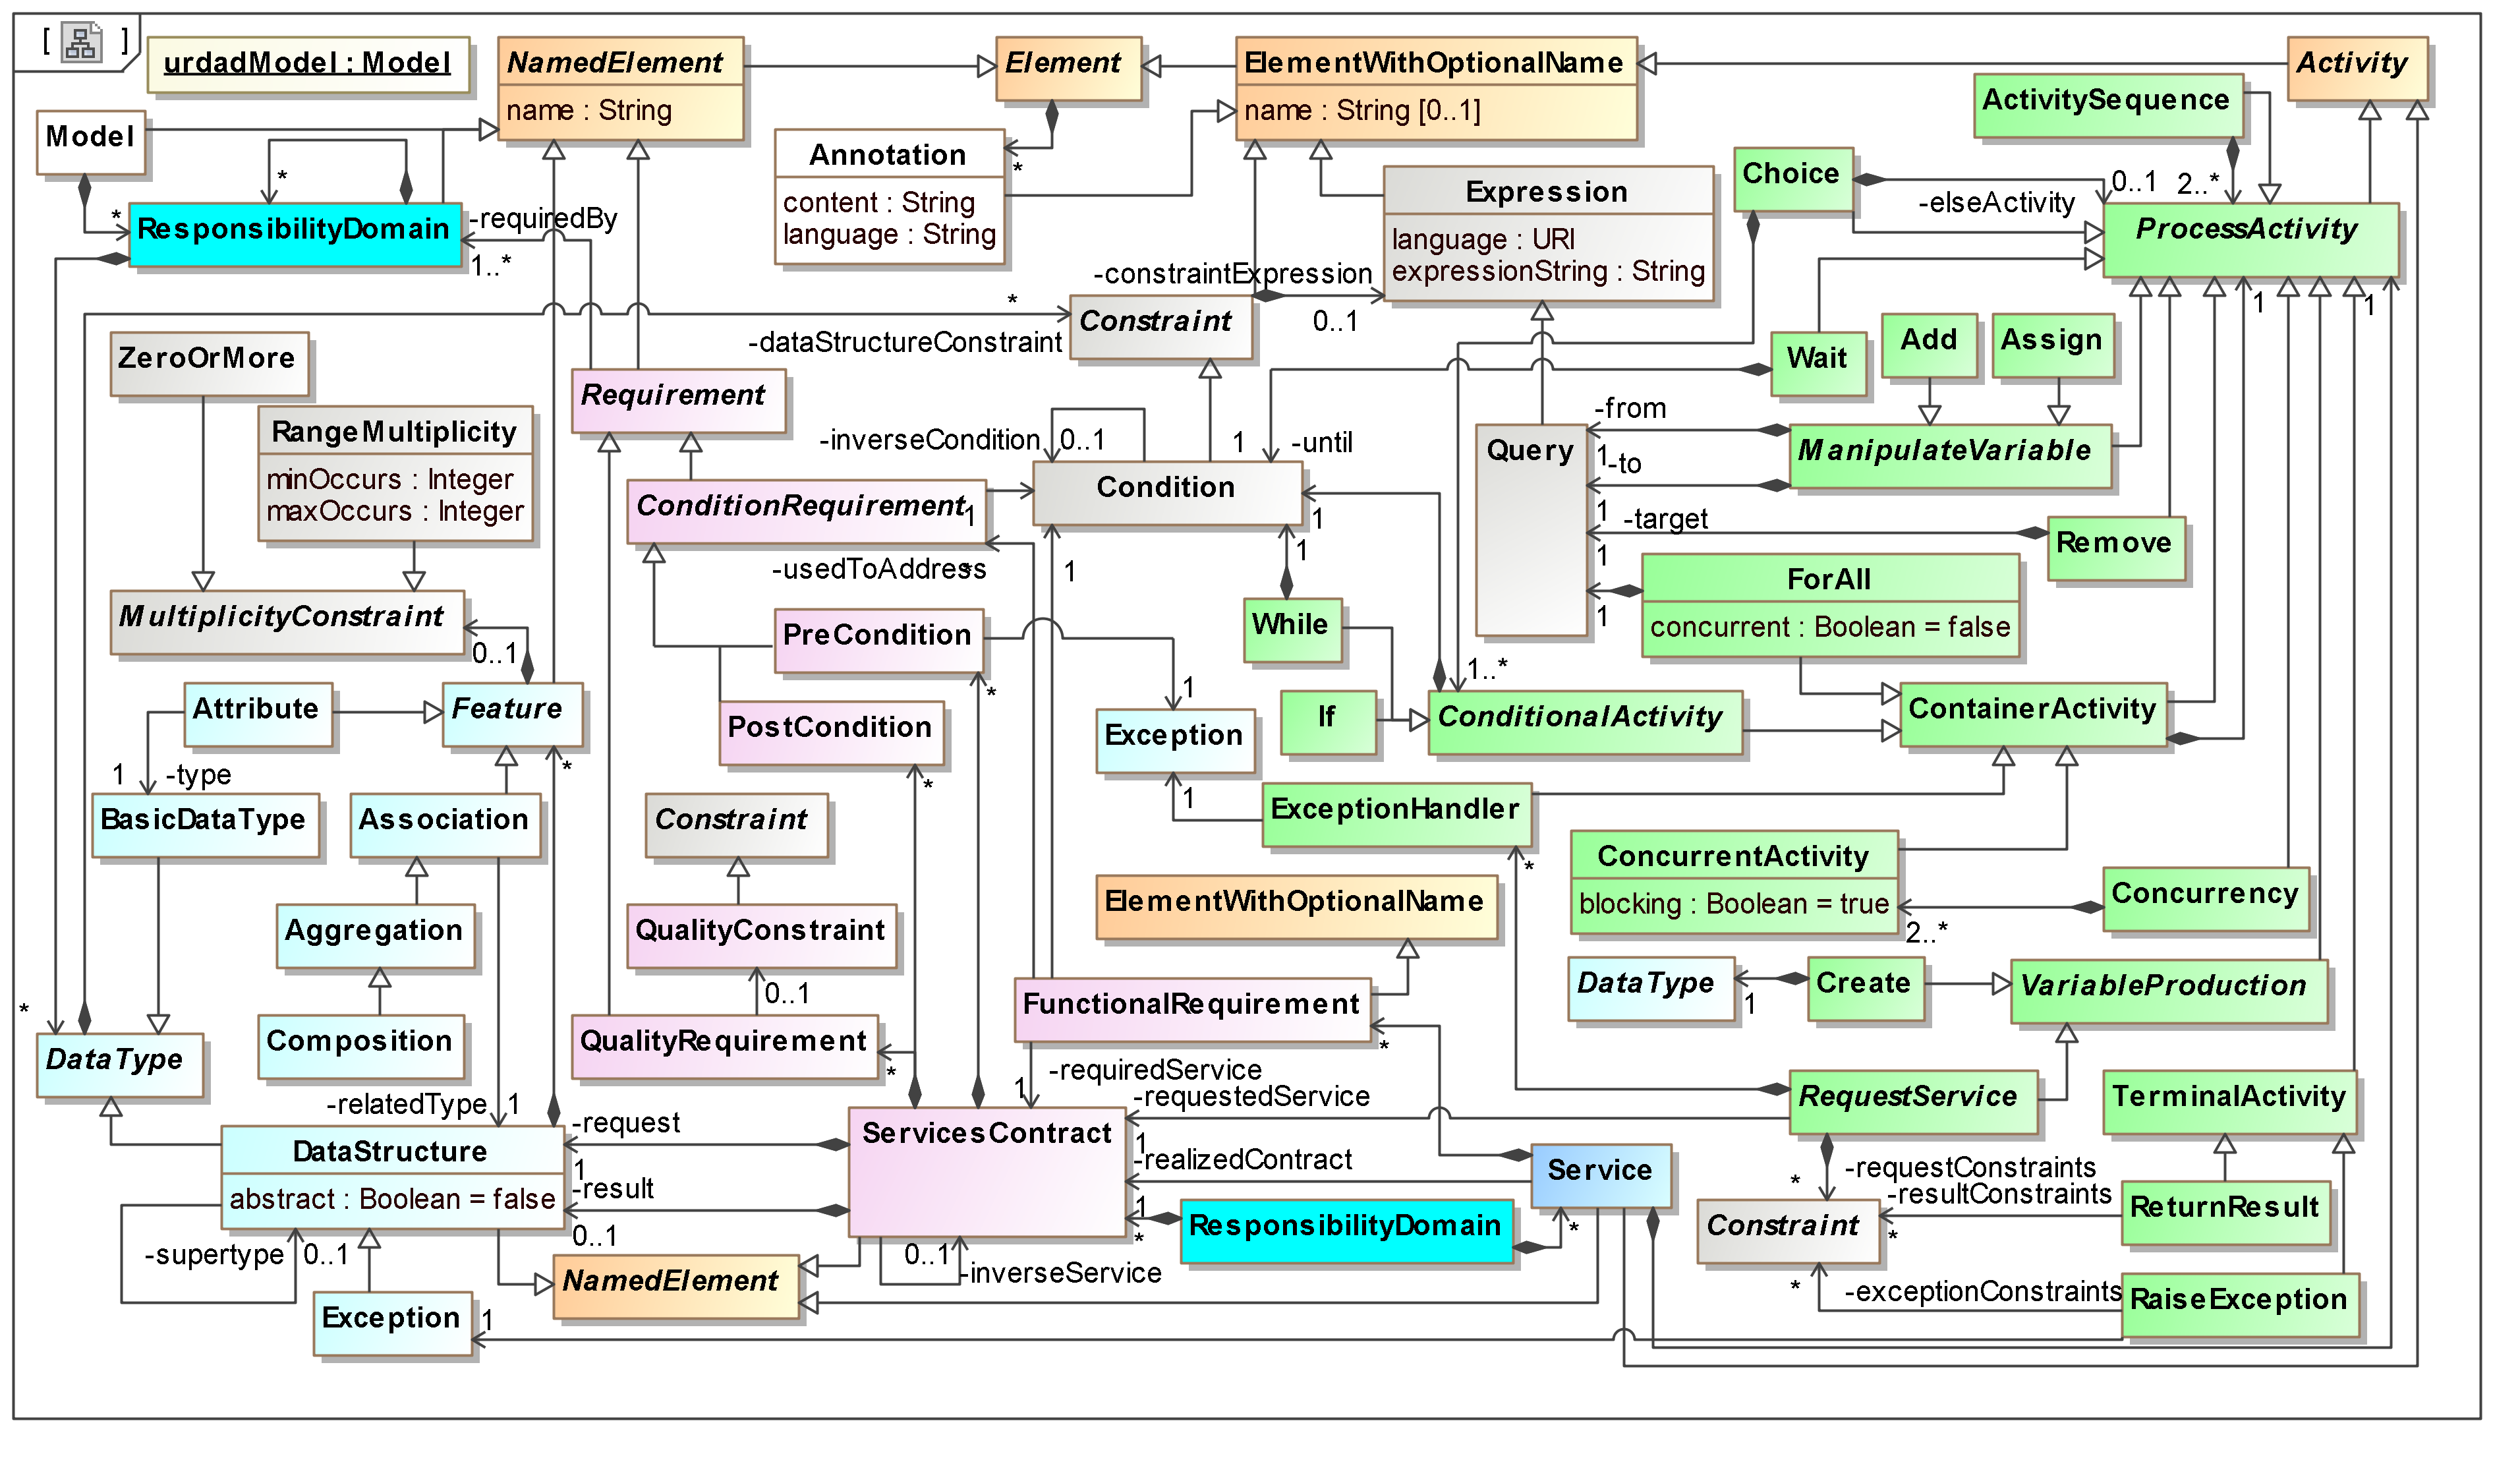
\includegraphics{metamodel}
  \caption{A diagrammatic representation of the URDAD metamodel}
  \label{fig:metamodel}
\end{figure}




\section{Provided artifacts}

The following artifacts are provided for th case study:
\begin{enumerate}
  \item this document,
  \item the Ecore file for the URDAD metamodel,
  \item a diagrammatic representation of the URDAD metamodel to speed up the understanding of the metamodel
  \item a concrete EMF-Text based text syntax for the URDAD DSL
  \item the use case for the case study in the form of both, 
    \begin{itemize}
     \item an XMI file, and
     \item in the concrete EMF-Text based text syntax.
    \end{itemize}
\end{enumerate}


\section{Use case description}

The provided use case is a typical business use case for enrolling a student for the presentation of a course. The target use case,
\verb+enrollForPresentation+ contains the specifications for the data structures for the request and result, the functional requirements
and the process specification which should enable the transformation team to generate the concrete implementation for that service
assembled from the required lower level services.


\begin{figure}
  \centering
  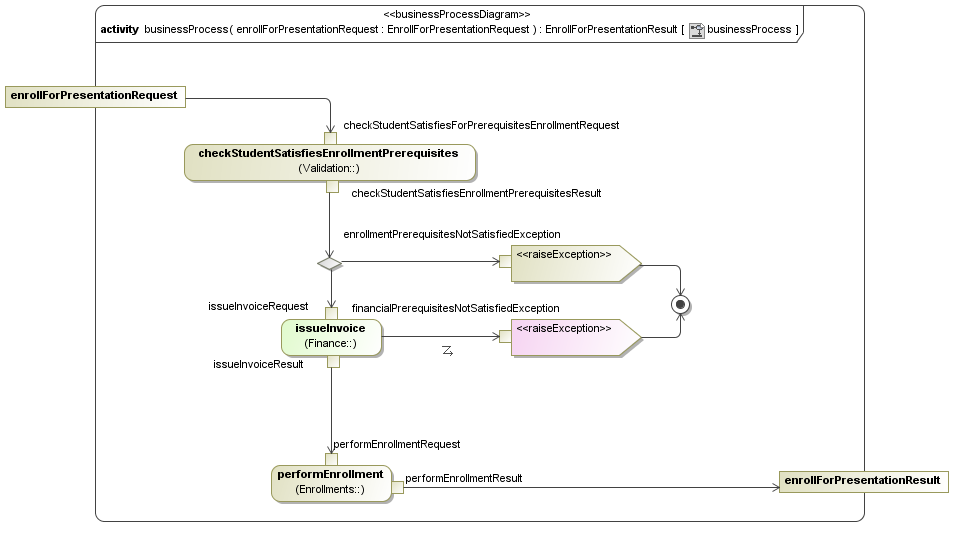
\includegraphics[width=\linewidth]{businessProcess}
  \caption{A diagrammatic representation of enrollForPresentation use case}
  \label{fig:businessProcess}
\end{figure}


\subsection{Subject modeled}

The input modeling language is the URDAD DSL. The metamodel specification and the example model are provided.

Since the model is meant to be a technology neutral model, the output modeling language is left up to the team and would correspond to the target technology chosen. This could be, for example, a model for either a JavaEE, Spring or SOA based implementation.

\subsection{Use case variation points}
Core use case variation points include
\begin{itemize}
  \item The implementation mapping for different architectures and technologies (e.g. implementaiton mapping onto SOA or JavaEE).
  \item Mapping of the URDAD model onto a UML model.
  \item Generation of UML diagrams showing the functional requirements, services contract and process specification.
\end{itemize}


\include{useCaseVariationPoints}

\section{Evaluation guidelines}

This section discusses 

\subsection{Mapping preferences}

When evaluating implementation mappings, we would recommend the following preferences, i.e. that the preferred mapping is rated higher than 
\begin{itemize}
  \item Declarative bi-directional mappings should be preferred over operational/algorithmic uni-directional mappings. 
  \item Standard mapping technologies like QVT relational should be preferred over custom mapping technologies.
  \item More simple, decoupled mapping rules should be preferred over fewer, complex rules.
  \item Standard target technologies commonly used for enterprise systems (e.g.\ JavaEE, SOA, Microsoft.Net) should be preferred over technologies seldom used for enterprise systems.
\end{itemize}

\subsection{Completeness measure}
The implementation should be tested against the tests developed or generated for the service contracts. 

Completeness checks should includes
\begin{itemize}
  \item whether the interfaces for the service contracts have been generated and to what extend they comply with the implementation guidelines,
  \item the completeness of the data structure specifications and the degree to which they confirm to the implementation guidelines,
  \item the completeness of the service implementations including whether
    \begin{itemize}
     \item the processes have been mapped onto method bodies,
     \item whether the request and result data structures are populated in the generated process specification,
     \item whether the conditionals for conditional flows and while loops are generated,
    \end{itemize}
  \item whether unit tests are generated from the service contracts and the completeness of the unit tests in the form of degree coverage of pre- and post-conditions.
\end{itemize}

\subsection{Correctness tests}

The correctness can be tested by assessing whether the service is realized in such a way that
\begin{itemize}
  \item if a particular precondition is not met, that the service is aborted raising that exception which was assigned in the model to that particular precondition.
  \item if all preconditions are met that the result object is obtained and all post-conditions evaluate to true after the service has been provided.
\end{itemize}

TODO: Add details
%       Correctness test: which are the reference input/ouput documents (models/graphs) and how should they be used? Ideally, a case description includes a testsuite, as well as a test driver
%             (The test driver can be an online web service, or a local script that can be deployed in Online demo in SHARE.)
% 
%           How to measure the quality of submitted solutions, at the design level?
%             (e.g., measure the number of rules, the conciseness of rules, ...)


\subsection{Systematic Evaluation Guidelines}
TODO: Add details

%     * How can the solutions be evaluated systematically using information technology?
%       Please provide one of the following:
%           a simple spreadsheet (an evaluation form that can be aggregated easily into an overview similar to this example table from 2010),
%           a so-called ?classification scheme? in ResearchR.org (or a similar web 2.0 platform.)


\section{Guidelines for the Implementation Mapping}

The following are some guidelines for the implementation mapping of specific URDAD model artifacts. The guidelines have a bias towards a typical modern object-oriented language like \verb+Java+ or \verb+C#+, but the concepts can be easily mapped onto other technologies.

\subsection{Responsibility domains}

Responsibility domains are meant to be mapped onto packages or name spaces as well as onto an interface with the name of the package with the capitalization converted to the convention of the target technology. 

\subsection{Service contracts}

Service contracts are meant to be mapped onto service/method declarations on interfaces or pure abstract classes which represent the services contract for a responsibility domain. The mapping of a contract for a specific service is meant to be done as follows:
\begin{itemize}
  \item The request object is an instance of a request class mapping onto a single input parameter is an instance of the request class,
  \item Both, the request and response/result classes are service specific and should, if the target technology supports it, be mapped onto static nested classes of the interface.
  \item If the target technology supports notifiable exceptions (e.g. Java), the exceptions raised for the preconditions of the service should be included in the throws clause of the service.
  \item If the target includes unit test generation, then the unit test for a service should test that
    \begin{itemize}
      \item the service is provided and not refused (no exception is thrown) if all pre-conditions are met,
      \item all post-conditions are satisfied after the service has been provided.
    \end{itemize}
\end{itemize}

\subsection{Service and process specification}

The concrete services in the metamodel contain the functional requirements (the lower level services from which the sevice is to be assembled) as well as the technology-neutral process specification which specifies how the process is orchestrated across these lower level services. There are service request activities, control structures, activities which create and manipulate local process variables and termination activities which either returning the result or notify the user that the requested service is not provided because a particular precondition for the service is not met by raising the exception associated with that precondition. 

The technology neutral design does not specify how references to the service providers of the lower level services are obtained. For modern implementation technologies this would typically be via dependency injection. The implementation mapping for other technologies might need to introduce a service provider registry and generate the approapriate service provider lookup code.

The process specification includes process variables which are accessible within the process and are maintained for the duration of the process. The inputs and outputs of the process (the request ond result objects for the core service itself) ae also process variables which can be queried and manipulated within the process.

\subsection{Data structures}

The URDAD data structure specification is essentially the same as in other object-oriented technologies supporting classes with attributes, association to other classes, inheritence and abstract classes. The different types of association relationships are meant to be implemented as follows:
\begin{itemize}
  \item Plain \textit{association} relationships are mapped onto simple references or pointers.
  \item \textit{Aggregation} relationships are implemented the same as plain association relationships except in the case where state change notification is to be supported. In these cases one also needs to ensure that the aggregate object listens to state change events from its components and that it issues the appropriate state change event to its observers.
  \item \textit{Composition} should be implemented as exclusive ownership, i.e. that the component is part of the owner and not part of any other object and should not survive the owner. Optionally the implementation mapping can implement full encapsulation for composition, i.e. that the component can only be accessed through the owner.
\end{itemize}


\subsection{Unit tests}

Unit tests should be developed for service contracts, not for concrete service definitions. They should only test the post-conditions for the current level of granularity, assuming that the lower level service providers fulfill their respective service contracts. In particular, they should test that
\begin{itemize}
  \item that the service is not refused if any of the preconditions do not hold true, i.e.\ that no exception is thrown, and
  \item that, when the service is provided (no exception thrown), all postconditions hold true after the service has been provided.
\end{itemize}



\bibliographystyle{plain}  %%abbrv
\bibliography{../../bibliography}

\end{document}

